\documentclass[tikz]{standalone}

% tikz
\usepackage{tikz, pgfplots}
% i wish external worked but idk it sucks
%\usetikzlibrary{external}
%\tikzexternalize[prefix=figures/]

% for function graph
\usetikzlibrary{positioning}
\usetikzlibrary{shapes.geometric}
\usetikzlibrary{positioning}
\usetikzlibrary{shapes.misc}
\tikzset{
dot/.style = {circle, fill=#1, minimum size=5pt,
              inner sep=0pt, outer sep=0pt},
dot/.default = black % size of the circle diameter
}
\tikzset{cross/.style={cross out, draw=black, minimum size=2*(#1-\pgflinewidth), inner sep=0pt, outer sep=0pt},
%default radius will be 1pt. 
cross/.default={1pt}}

\usetikzlibrary{ducks} % ducks :))

 % for braces
\usetikzlibrary{decorations.pathreplacing}
% for hashing area
\usetikzlibrary{patterns}
% tableaux var, signe
% source https://www.sqlpac.com/fr/documents/latex-package-tkz-tab-tikz-tableaux-de-signes-et-de-variations-de-fonctions.html
\usepackage{tkz-tab}

%%%%%%%%%%%%%%%%%%%%%%%%%%%%%%
% SELF MADE COLORS
%%%%%%%%%%%%%%%%%%%%%%%%%%%%%%


\definecolor{myg}{RGB}{56, 140, 70}
\definecolor{myb}{RGB}{45, 111, 177}
\definecolor{myr}{RGB}{199, 68, 64}
\definecolor{mytheorembg}{HTML}{F2F2F9}
\definecolor{mytheoremfr}{HTML}{00007B}
\definecolor{mylenmabg}{HTML}{FFFAF8}
\definecolor{mylenmafr}{HTML}{983b0f}
\definecolor{mypropbg}{HTML}{f2fbfc}
\definecolor{mypropfr}{HTML}{191971}
\definecolor{myexamplebg}{HTML}{F2FBF8}
\definecolor{myexamplefr}{HTML}{88D6D1}
\definecolor{myexampleti}{HTML}{2A7F7F}
\definecolor{mydefinitbg}{HTML}{E5E5FF}
\definecolor{mydefinitfr}{HTML}{3F3FA3}
\definecolor{notesgreen}{RGB}{0,162,0}
\definecolor{myp}{RGB}{197, 92, 212}
\definecolor{mygr}{HTML}{2C3338}
\definecolor{myred}{RGB}{127,0,0}
\definecolor{myyellow}{RGB}{169,121,69}
\definecolor{myexercisebg}{HTML}{F2FBF8}
\definecolor{myexercisefg}{HTML}{88D6D1}
\definecolor{doc}{RGB}{0,60,110}

% manim colors because they're beautiful
% https://docs.manim.community/en/stable/reference/manim.utils.color.manim_colors.html

\definecolor{BLACK}{HTML}{000000}\definecolor{BLUE}{HTML}{58C4DD}\definecolor{BLUE_A}{HTML}{C7E9F1}\definecolor{BLUE_B}{HTML}{9CDCEB}\definecolor{BLUE_C}{HTML}{58C4DD}\definecolor{BLUE_D}{HTML}{29ABCA}\definecolor{BLUE_E}{HTML}{236B8E}\definecolor{DARKER_GRAY}{HTML}{222222}\definecolor{DARKER_GREY}{HTML}{222222}\definecolor{DARK_BLUE}{HTML}{236B8E}\definecolor{DARK_BROWN}{HTML}{8B4513}\definecolor{DARK_GRAY}{HTML}{444444}\definecolor{DARK_GREY}{HTML}{444444}\definecolor{GOLD}{HTML}{F0AC5F}\definecolor{GOLD_A}{HTML}{F7C797}\definecolor{GOLD_B}{HTML}{F9B775}\definecolor{GOLD_C}{HTML}{F0AC5F}\definecolor{GOLD_D}{HTML}{E1A158}\definecolor{GOLD_E}{HTML}{C78D46}\definecolor{GRAY}{HTML}{888888}\definecolor{GRAY_A}{HTML}{DDDDDD}\definecolor{GRAY_B}{HTML}{BBBBBB}\definecolor{GRAY_BROWN}{HTML}{736357}\definecolor{GRAY_C}{HTML}{888888}\definecolor{GRAY_D}{HTML}{444444}\definecolor{GRAY_E}{HTML}{222222}\definecolor{GREEN}{HTML}{83C167}\definecolor{GREEN_A}{HTML}{C9E2AE}\definecolor{GREEN_B}{HTML}{A6CF8C}\definecolor{GREEN_C}{HTML}{83C167}\definecolor{GREEN_D}{HTML}{77B05D}\definecolor{GREEN_E}{HTML}{699C52}\definecolor{GREY}{HTML}{888888}\definecolor{GREY_A}{HTML}{DDDDDD}\definecolor{GREY_B}{HTML}{BBBBBB}\definecolor{GREY_BROWN}{HTML}{736357}\definecolor{GREY_C}{HTML}{888888}\definecolor{GREY_D}{HTML}{444444}\definecolor{GREY_E}{HTML}{222222}\definecolor{LIGHTER_GRAY}{HTML}{DDDDDD}\definecolor{LIGHTER_GREY}{HTML}{DDDDDD}\definecolor{LIGHT_BROWN}{HTML}{CD853F}\definecolor{LIGHT_GRAY}{HTML}{BBBBBB}\definecolor{LIGHT_GREY}{HTML}{BBBBBB}\definecolor{LIGHT_PINK}{HTML}{DC75CD}\definecolor{LOGO_BLACK}{HTML}{343434}\definecolor{LOGO_BLUE}{HTML}{525893}\definecolor{LOGO_GREEN}{HTML}{87C2A5}\definecolor{LOGO_RED}{HTML}{E07A5F}\definecolor{LOGO_WHITE}{HTML}{ECE7E2}\definecolor{MAROON}{HTML}{C55F73}\definecolor{MAROON_A}{HTML}{ECABC1}\definecolor{MAROON_B}{HTML}{EC92AB}\definecolor{MAROON_C}{HTML}{C55F73}\definecolor{MAROON_D}{HTML}{A24D61}\definecolor{MAROON_E}{HTML}{94424F}\definecolor{ORANGE}{HTML}{FF862F}\definecolor{PINK}{HTML}{D147BD}\definecolor{PURE_BLUE}{HTML}{0000FF}\definecolor{PURE_GREEN}{HTML}{00FF00}\definecolor{PURE_RED}{HTML}{FF0000}\definecolor{PURPLE}{HTML}{9A72AC}\definecolor{PURPLE_A}{HTML}{CAA3E8}\definecolor{PURPLE_B}{HTML}{B189C6}\definecolor{PURPLE_C}{HTML}{9A72AC}\definecolor{PURPLE_D}{HTML}{715582}\definecolor{PURPLE_E}{HTML}{644172}\definecolor{RED}{HTML}{FC6255}\definecolor{RED_A}{HTML}{F7A1A3}\definecolor{RED_B}{HTML}{FF8080}\definecolor{RED_C}{HTML}{FC6255}\definecolor{RED_D}{HTML}{E65A4C}\definecolor{RED_E}{HTML}{CF5044}\definecolor{TEAL}{HTML}{5CD0B3}\definecolor{TEAL_A}{HTML}{ACEAD7}\definecolor{TEAL_B}{HTML}{76DDC0}\definecolor{TEAL_C}{HTML}{5CD0B3}\definecolor{TEAL_D}{HTML}{55C1A7}\definecolor{TEAL_E}{HTML}{49A88F}\definecolor{WHITE}{HTML}{FFFFFF}\definecolor{YELLOW}{HTML}{FFFF00}\definecolor{YELLOW_A}{HTML}{FFF1B6}\definecolor{YELLOW_B}{HTML}{FFEA94}\definecolor{YELLOW_C}{HTML}{FFFF00}\definecolor{YELLOW_D}{HTML}{F4D345}\definecolor{YELLOW_E}{HTML}{E8C11C}

% Schwartz
\renewcommand{\S}{\mathcal{S}} % \S est le signe paragraphe normalement

% corps
\newcommand{\C}{\mathcal{C}}
\newcommand{\R}{\mathbb{R}}
\newcommand{\Rnn}{\mathbb{R}^{2n}}
\newcommand{\Z}{\mathbb{Z}}
\newcommand{\N}{\mathbb{N}}
\newcommand{\Q}{\mathbb{Q}}

% domain
\newcommand{\D}{\mathcal{D}}

% order notations
\renewcommand{\O}{\mathcal{O}}

% japanese bracket
\newcommand{\japb}[1]{\langle #1 \rangle}

% arrows over partial derivatives
\newcommand{\lp}{\overleftarrow{\partial}}
\newcommand{\rp}{\overrightarrow{\partial}}

% quantization
\newcommand{\h}{\hbar}
\newcommand{\Opht}{\textrm{Op}_{\h}^{t}}
\newcommand{\Op}[2][\hbar]{\textrm{Op}_{#1}^{#2}}

% omega functions
\newcommand{\omegap}[2][\rho_0]{\omega(\partial_{#1},\partial_{#2})}
\newcommand{\omegar}[2][\rho_0]{\omega(#1,#2)}

\newcommand{\pvec}[2]{
	\begin{pmatrix}#1 \\ #2 \end{pmatrix}
}

\begin{document}
%
	% page 1
	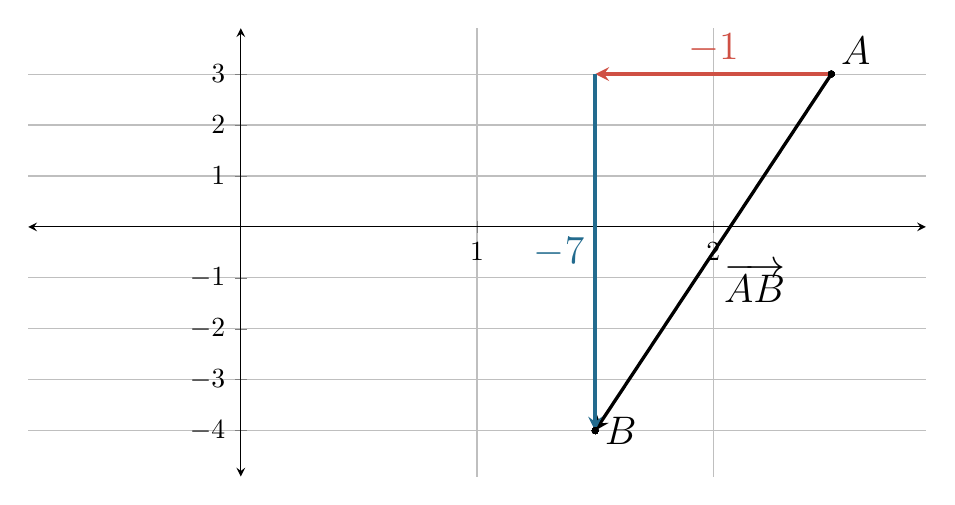
\begin{tikzpicture}[>=stealth, scale=1]
	\begin{axis}[xmin = -0.9, xmax=2.9, xtick={ -3, ..., 5}, ymin=-4.9, ymax=3.9, axis x line=middle, axis y line=middle, axis line style=<->, xlabel={}, ylabel={}, ytick = {-4, -3, ..., 2, 3}, grid=both, x=3cm]
		
		\addplot[black, mark=*, mark size = 1] (2.5,3) node[above right, font=\Large] {$A$};
		\addplot[black, mark=*, mark size = 1] (1.5,-4) node[right, font=\Large] {$B$};
	
		\draw[very thick, black, ->] (axis cs:2.5,3) -- (axis cs:1.5,-4) node[below right, pos=.5, font=\Large] {$\overrightarrow{AB}$};
		\draw[very thick, RED_E, ->] (axis cs:2.5,3) -- (axis cs:1.5,3) node[above, pos=.5, font=\Large] {$-1$};
		\draw[very thick, BLUE_E, ->] (axis cs:1.5,3) -- (axis cs:1.5,-4) node[left, pos=.5, font=\Large] {$-7$};
	\end{axis}
	\end{tikzpicture}
	%page 2
	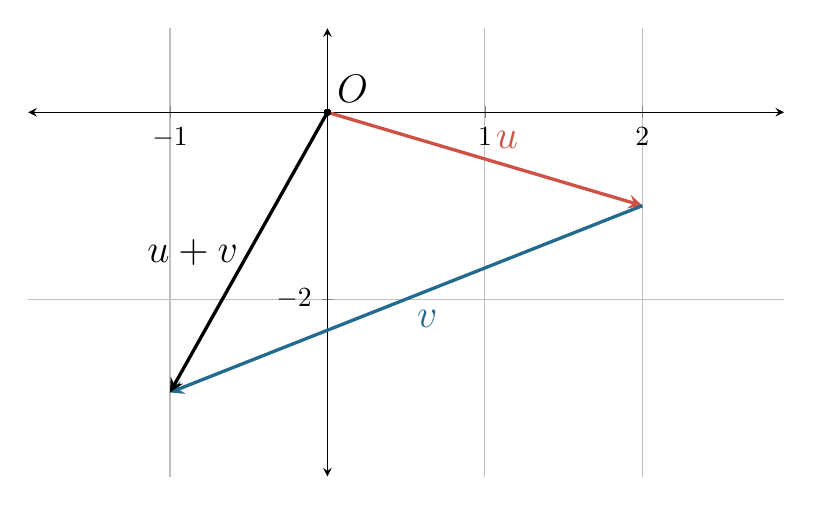
\begin{tikzpicture}[>=stealth, scale=1]
	\begin{axis}[xmin = -1.9, xmax=2.9, xtick={ -3, ..., 5}, ymin=-3.9, ymax=0.9, ytick={-2}, axis x line=middle, axis y line=middle, axis line style=<->, xlabel={}, ylabel={}, grid=both, x=2cm]
		
		\addplot[black, mark=*, mark size = 1] (0,0) node[above right, font=\Large] {$O$};
	
		\draw[very thick, RED_E, ->] (axis cs:0, 0) -- (axis cs:2, -1) node[above right, pos=.5, font=\Large] {$u$};
		
		\draw[very thick, BLUE_E, ->] (axis cs:2, -1) -- (axis cs:-1, -3) node[below right, pos=.5, font=\Large] {$v$};
		
		\draw[very thick, black, ->] (axis cs:0, 0) -- (axis cs:-1, -3) node[left, pos=.5, font=\Large] {$u+v$};
	\end{axis}
	\end{tikzpicture}
	% page 3
	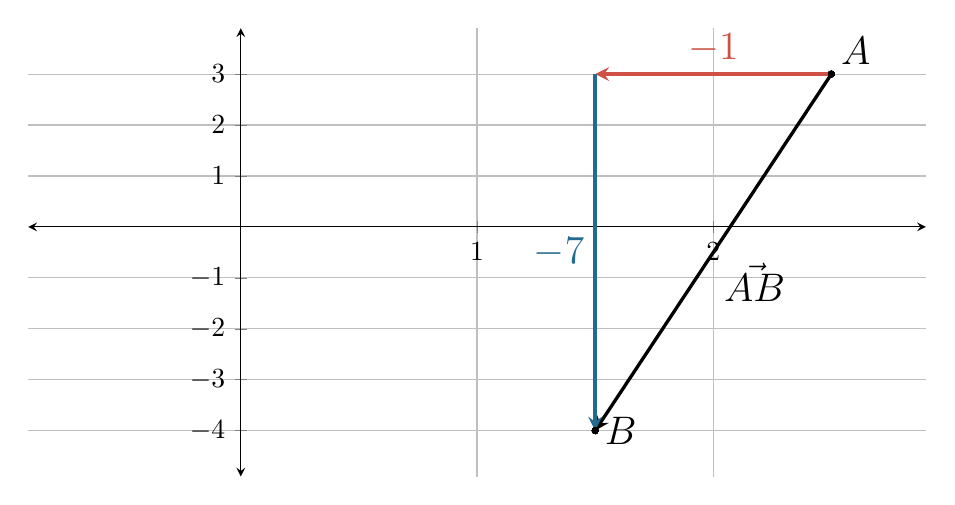
\begin{tikzpicture}[>=stealth, scale=1]
	\begin{axis}[xmin = -0.9, xmax=2.9, xtick={ -3, ..., 5}, ymin=-4.9, ymax=3.9, axis x line=middle, axis y line=middle, axis line style=<->, xlabel={}, ylabel={}, ytick = {-4, -3, ..., 2, 3}, grid=both, x=3cm]
		
		\addplot[black, mark=*, mark size = 1] (2.5,3) node[above right, font=\Large] {$A$};
		\addplot[black, mark=*, mark size = 1] (1.5,-4) node[right, font=\Large] {$B$};
	
		\draw[very thick, black, ->] (axis cs:2.5,3) -- (axis cs:1.5,-4) node[below right, pos=.5, font=\Large] {$\vec{AB}$};
		\draw[very thick, RED_E, ->] (axis cs:2.5,3) -- (axis cs:1.5,3) node[above, pos=.5, font=\Large] {$-1$};
		\draw[very thick, BLUE_E, ->] (axis cs:1.5,3) -- (axis cs:1.5,-4) node[left, pos=.5, font=\Large] {$-7$};
	\end{axis}
	\end{tikzpicture}
	
	% page 4
	\begin{tikzpicture}
	\scope
		\clip 
		(-6.5,-4.5) rectangle (6.5,4.5)
		(-6.5,2) -- (-6.5,-4.5)  -- (4,-4.5) -- cycle;
		\draw[step=1,gray, thin, opacity=.5] (-6.5,-4.5) grid (6.5,4.5);
	\endscope
	
	\draw (-6,2.5) pic[
		scale=.75,
		duck/glasses,
		  duck/bookcolour=black!60!brown,
		  duck/book={
		      \scalebox{0.14}{
		      \parbox{2.5cm}{
		      \sffamily
		      \centering
		      \footnotesize
		      $1+1=2$}}},
		  duck/strawhat
	] {duck};
	
	\draw[very thick, ->, PURPLE_E] (-3.75,3.25) -- (3.75,3.25) node[midway, below, font=\huge] {$x_T$};
	
	\draw (4.5,2.5) pic[
		scale=.75,
		duck/glasses,
		  duck/bookcolour=black!60!brown,
		  duck/book={
		      \scalebox{0.14}{
		      \parbox{2.5cm}{
		      \sffamily
		      \centering
		      \footnotesize
		      $1+1=2$}}},
		  duck/strawhat
	] {duck};
	
	\draw[very thick, ->, RED_E] (5.25,2.5) -- (5.25,-1.5) node[midway, left, font=\huge] {$y_T$};
	
	\draw (4.5,-3.5) pic[
		scale=.75,
		duck/glasses,
		  duck/bookcolour=black!60!brown,
		  duck/book={
		      \scalebox{0.14}{
		      \parbox{2.5cm}{
		      \sffamily
		      \centering
		      \footnotesize
		      $1+1=2$}}},
		  duck/strawhat
	] {duck};
	
	\draw[very thick, ->] (-4.2,2.8) -- (4.5,-2.5) node[midway, below left, font=\huge] {$T$};
	
	\node[, font=\huge] at (-3,-3) {
		$\begin{aligned}
		T &= \pvec{\color{PURPLE_E}x_T}0 + \pvec0{\color{RED_E}y_T} \\
			&= \pvec{\color{PURPLE_E}x_T}{\color{RED_E}y_T}
		\end{aligned}$
	};
	
	\end{tikzpicture}
%
\end{document}